\section{The ATLAS Detector}

ATLAS is one of the two general purpose detectors built for probing proton-proton 
collision. This detector represents the work of a large collaboration 
of several thousand physicists, engineers, technicians,
and students over a period of fifteen years of dedicated 
design, development, fabrication, and installation.
The overall layout of the detector is shown in Figure~\ref{fig:ATLAS_cut_away}~\cite{PERF-2007-01}.
It has the shape of a cylinder, 46~m long, 25~m in diameter, 
and sits in a cavern 100~m below ground. The ATLAS detector weighs 7000 tonnes, 
similar to the weight of the Eiffel Tower.
The detector itself is a many-layered instrument designed to detect some 
of most energetic particles ever created on earth. 
It consists of six different detecting subsystems wrapped concentrically 
in layers around the collision point of nearly 4$\pi$ solid angle coverage
to record the trajectory, momentum, and energy of particles, 
allowing them to be individually identified and measured. 
These six subsystems are 
the pixel detector~\cite{ATLAS-TDR-11}, 
the semiconductor tracker (SCT)~\cite{ATLAS-TDR-04}, 
the transition radiation tracker (TRT)~\cite{ATLAS-TDR-04},
the electromagnetic (EM) calorimeter~\cite{ATLAS-TDR-02}, 
the hadronic calorimeter~\cite{ATLAS-TDR-03}
and the muon spectrometer (MS)~\cite{ATLAS-TDR-10}.
The first three sub-detectors are collectively known as the inner detector (ID),
described in section~\ref{sec:inner detector}, and it is used for tracking charged particles. 
The electromagnetic and the hadronic calorimeter, described in section~\ref{sec:calorimeter},
are responsible for measuring the energies of the electromagnetic and hadronic particles respectively. 
The MS, described in section~\ref{sec:MS}, is a unique sub-detector used for measuring the 
momentum of muons leaving the calorimeters.

A huge magnet system bends the paths of the charged particles so that their 
momenta can be measured as precisely as possible.

\begin{figure}[bht]
\begin{centering}	
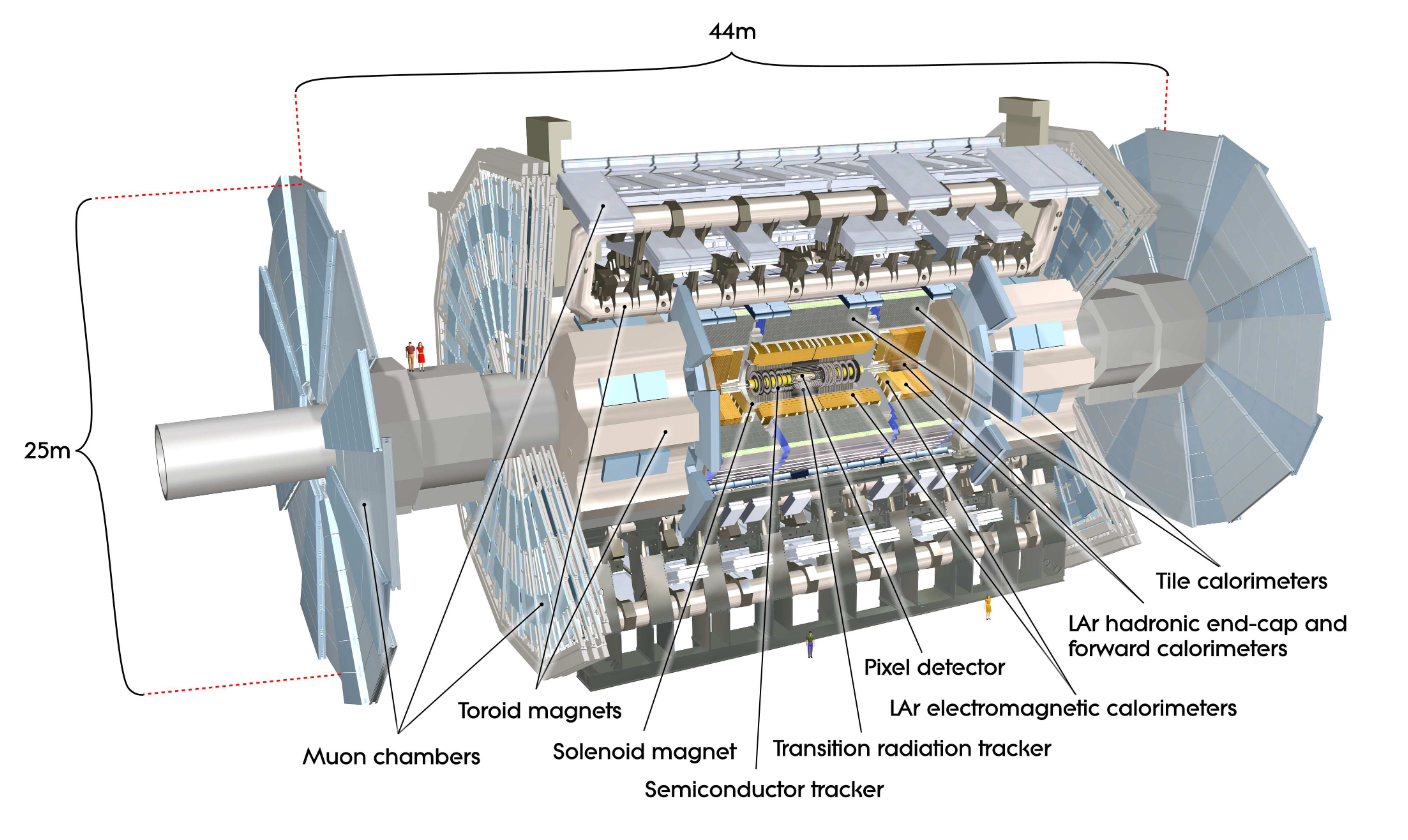
\includegraphics[width=1.0\textwidth]{Detector/plots/Cut-away-view-of-the-ATLAS-detector.png}
\caption{Cut-away view of the ATLAS detector. 
The dimensions of the detector are 25~m in
height and 44~m in length. The overall weight 
of the detector is approximately 7000 tonnes. The figure is taken from reference \cite{PERF-2007-01}.
	}
\label{fig:ATLAS_cut_away}
\end{centering}
\end{figure}

The high interaction rates, radiation doses, particle multiplicities 
and energies, as well as the requirements for precision measurements 
have set strigent standards on the design of the ATLAS detector. 
Therefore the ATLAS detector is designed to fufiled the following 
requirements:

\begin{itemize}
\item
Fast, radiation-resistant electronics and sensor elements 
and high detector granularity. This is due to the
 high frequency of collisions, high particle fluxes and 
 high radiation environment of the detector.
\item
Large acceptance in polar angle with almost full azimuthal angle coverage,
due to the geometry of the detector 
(more details in section~\ref{sec:detector coordinate}).
\item
Good energy resolution calorimetry, as required to 
enable accurate physical object reconstruction. 
The high resolution of energy can be obtained 
with very good electromagnetic calorimetry for 
electron and photon identification and measurements,
complemented by full-coverage hadronic calorimetry 
for accurate jet and missing transverse energy measurements.
\item  
Tracking of precision in the ID, as required to provide high momentum 
resolution and to allow the reconstruction of
secondary vertices to identify $b$-hadrons and $\tau$-leptons.
\item
Good muon identification and momentum resolution 
over a wide range of momenta and the ability 
to determine unambiguously the charge of high-\pt\ 
muons in the muon spectrometer.
\item
Trigger system with high efficiency on low \pt\  
objects with sufficient background rejection, 
which is a prerequisite to achieve an acceptable trigger rate 
for most physics processes of interest.
\end{itemize}


The main performance goals of the detector are 
listed in Table \ref{tab:ATLAS_performance}. 
\begin{table}[thb]
	\centering
	\small
	\setlength\tabcolsep{5pt} 
	\begin{tabular}{|l|l|l|l| }
	\hline
	\multirow{2}{*}{Detector component}&\multirow{2}{*}{Required resolution} & \multicolumn{2}{l|}{$\eta$ coverage} \\ \cline{3-4}
	
	  & & Measurement &  Trigger\\ 
	 \hline
	Tracking         &    $\sigma_{p_T}/p_T = 0.05\%\ p_T\bigoplus 1\% $        &  $\pm 2.5$  & None \\  
	\hline
	EM calorimetry      &  $\sigma_E/E = 10\%\ /E\bigoplus 0.7\% $       & $\pm 3.2$ &  $\pm 2.5$\\
	\hline
	Hadronic calorimetry  &        & &      \\
	% \hline
	\ \ barrel and end-cap &  $\sigma_E/E = 50\%/E\bigoplus 3\% $       & $\pm 3.2$ &  $\pm 3.2$\\
	\ \ forward   &  $\sigma_E/E = 100\%\ /E\bigoplus 10\% $       & $ 3.1 < |\eta | < 4.9 $ &  $3.1 < |\eta | < 4.9 $\\
	\hline
	Muon spectrometer  &    $\sigma_{p_T}/p_T = 10\%$ at \pt $=\ 1$ TeV        &  $\pm 2.7$  & $\pm 2.4$ \\  
	\hline
	\end{tabular}
	\vspace{0.2cm}
	\caption{General performance goals of the ATLAS detector. The units for energy of the particle, E
	and transverse momentum, \pt\ (detailed definition in section~\ref{sec:detector coordinate}) 
	are in GeV~\cite{PERF-2007-01}. Note that, for high-\pt\ muons,
	the muon-spectrometer performance is independent of the inner-detector system.}
	\label{tab:ATLAS_performance}
\end{table}



\subsection{Coordinate system}
\label{sec:detector coordinate}

The ATLAS coordinate system is a right-handed Cartesian system
with the nominal interaction point 
defined as the origin of the coordinate system,  
while the beam direction defines the $z$-axis and 
the $x$-$y$ plane is transverse to the beam direction.  
The positive $x$-axis is defined as pointing from 
the interaction point to the centre of the
LHC ring and the positive $y$-axis is defined as 
pointing upwards, as shown in Figure~\ref{fig:ATLAS_coordinate_system}. 

\begin{figure}[bht]
	\begin{centering}	
	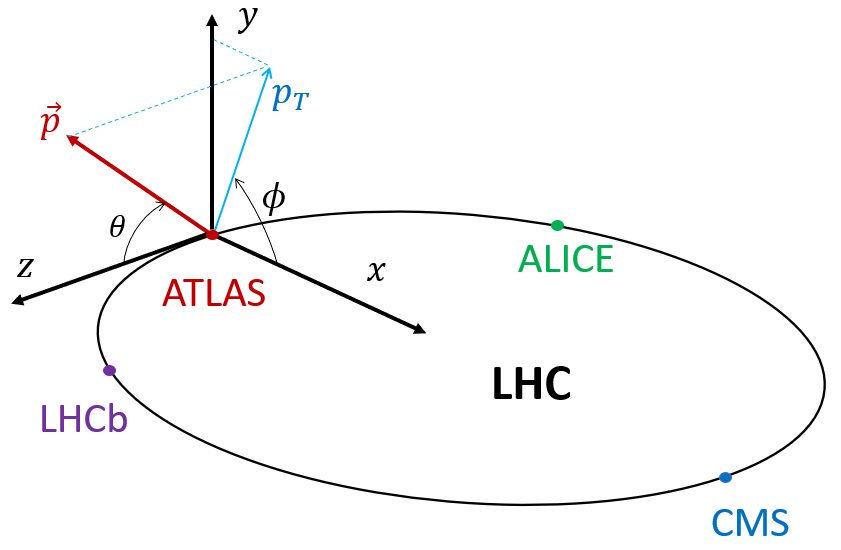
\includegraphics[width=.75\textwidth]{Detector/plots/ATLAS coordinate system.png}
	\caption{Illustration of the coordinate system
	used at the ATLAS experiment in the geographical context of the LHC.
		}
	\label{fig:ATLAS_coordinate_system}
	\end{centering}
\end{figure}

The azimuthal angle $\phi$ 	is measured as usual around the beam axis, 
and the polar angle $\theta$ is the angle from the beam axis.  
In high energy physics, it's more common to use the 
pseudorapidity instead of the polar angle $\theta$, defined as:
\[
		\eta = -\ln\ \tan(\theta/2). 
\]
In the case of highly relativistic particles
(which is the comman case in high energy physics), 
the pseudorapidity approaches the rapidity, 
\[ 
	y=1/2\ln[(E+p_z)/(E-p_z)], 
\]
where $E$ is the energy of the particle, $m$ is its mass 
and $p_z$ is the momentum along the $z$-axis.
There are two main reasons for using pseudorapidity 
rather than the polar angle $\theta$ nor the rapidity.
The reason for using pseudorapidity but not $\theta$ 
is that the rapidity is invariant
under Lorentz transformation, while capturing 
the characteristic of the particle direction of travel:
$y \rightarrow \pm \infty $ when the particle is  
travelling close to the beam pipe (positive for along the
beam pipe, negative for the opposite direction) and
$y \rightarrow 0$ when $p_z$ is small.
The reason for using pseudorapidity but not rapidity
is that due to the limited angle coverage of the detector, 
it's usually hard to determine the total energy and the momentum 
along the $z$-axis, especially when the direction of 
the particles are close to the beam pipe. 
While the pseudorapidity is determined only by
the polar angle, which is much easier and faster 
to compute. 
Another commonly used variable, transverse momentum \pt, 
is defined as the momentum of a particle transverse to the 
beam direction ($z$-direction):
\[ 
	\vec{p_T}= (p_x,p_y).
\]
The reason for using transverse momentum 
is that, because the partons that make up a proton share the momentum,
the initial longitudinal momentum is unknown;	
we do know, however, that the initial transverse momentum was zero. 
And hence we can look for the missing transverse momentum, defined
as 
\[ 
	\vec{E_T}^{miss}=-\sum_i \vec{p_{T_i}} \label{eq:MET}
\]
for visible particles $i$, where \met\ is the magnitude of $\vec{E_T}^{miss}$
 (Confusingly $E_T^{miss}$ is commonly called 
missing transverse energy or MET. Missing transverse energy is equivalent 
to missing transverse momentum only if the missing particle(s) were massless.). 
Finnaly, the distance $\Delta R$ in the pseudorapidity-azimuthal angle 
space is defined as:
\[\Delta R = \sqrt{\Delta \eta^2+\Delta\phi^2},\]
where $R$ is the radial distance from the particle position to the interaction 
vertex.

\subsection{Magnets}


ATLAS has a unique hybrid system of four large superconducting 
magnets~\cite{ATLAS-TDR-06}. This magnetic system is 22~m in diameter and 26~m in length, 
with a stored energy of 1.6~GJ. Figure~\ref{fig:ATLAS_magnets_site} shows the real scale of
the magnets system compared to a person. 
Figure~\ref{fig:ATLAS_cut_away} shows the general layout, 
the four main layers of detetors and the four superconducting 
magnets which provide the magnetic
field over a volume of approximately 12000~m$^3$.



\begin{figure}[bht]
	\begin{centering}	
	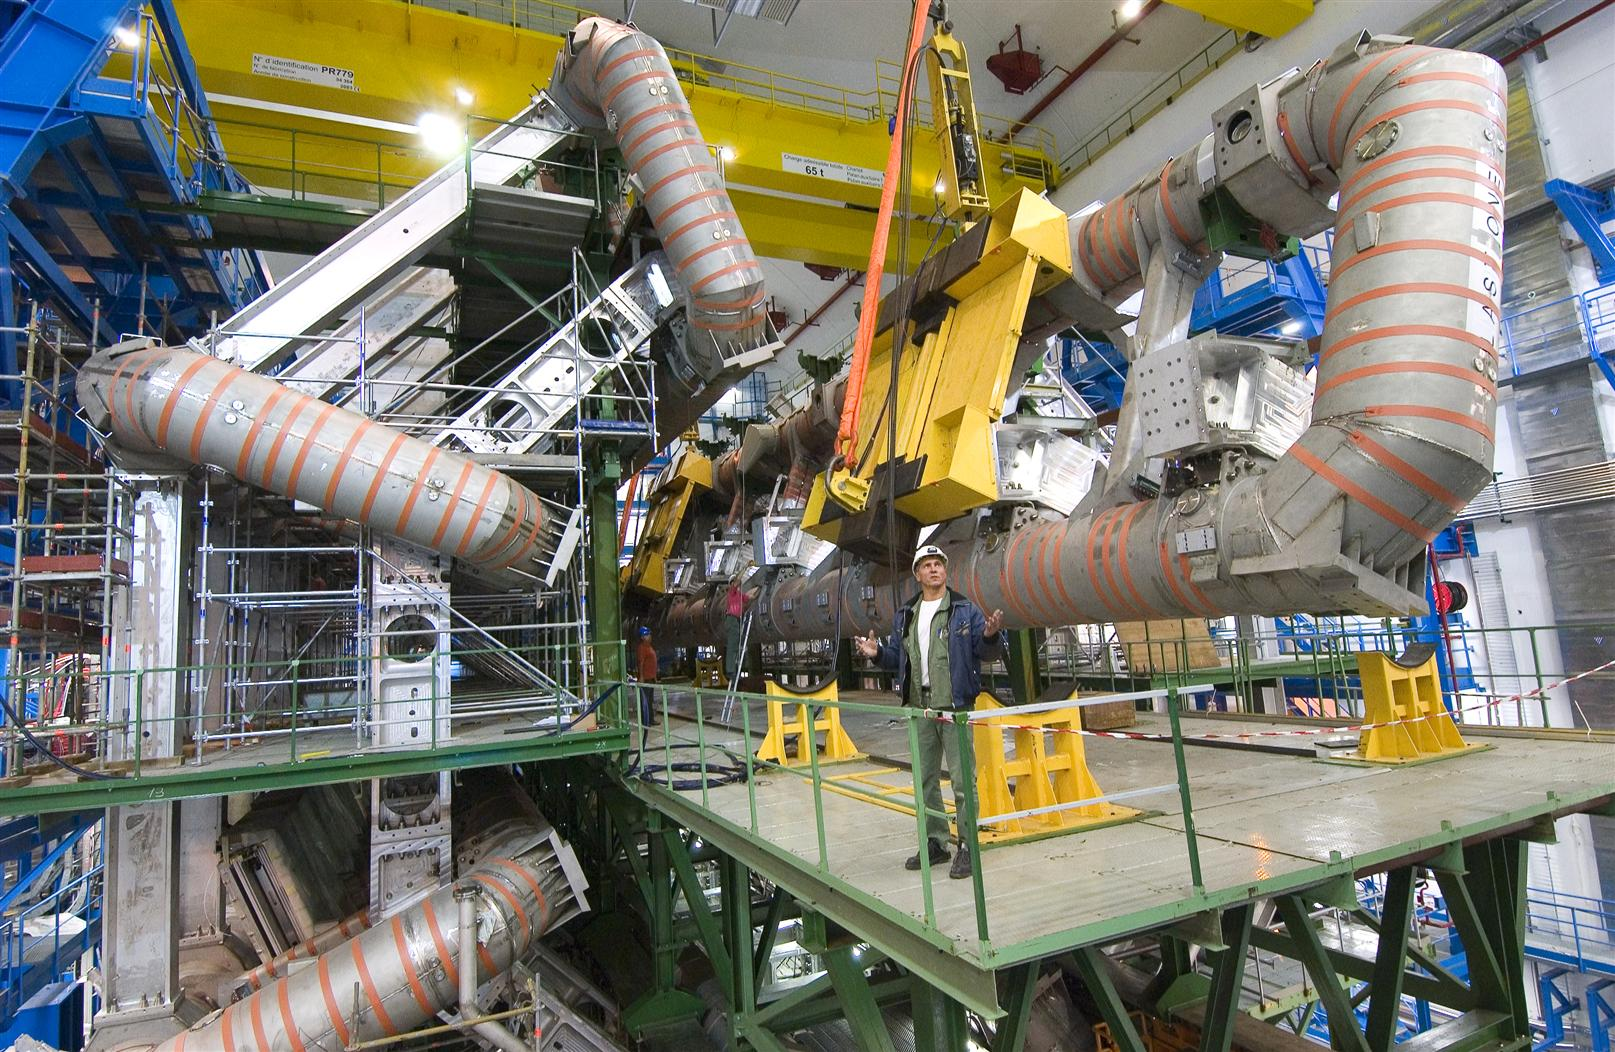
\includegraphics[width=.8\textwidth]{Detector/plots/magnets.jpg}
	\caption{A picture showing the real size magnets compared to a person.}
	\label{fig:ATLAS_magnets_site}
	\end{centering}
\end{figure}




The spatial arrangement of the coil windings is shown in 
Figure~\ref{fig:ATLAS_magnets}. 
The ATLAS magnet system consists of two parts:
\begin{itemize}
	\item a solenoid, which is aligned on the beam axis and 
	provides a 2 T axial magnetic field in the $z$-direction
	for the ID. Becasue the magnet is located in front
	of the EM calorimeter, it is imperative to minimise possible interactions
	between the magnet and the particles being studied.
	This is achieved by embedding over 9 km of niobium-titanium 
	superconductor wires into strengthened, pure aluminum strips, 
	which is capable to provide such powerful magnetic field
	in just 4.5 cm thickness. 
	% while minimising the radiative thickness in front of the	barrel 
	% electromagnetic calorimeter;
	\item  A barrel toroid and two end-cap toroids, 
	which produce a	toroidal magnetic field of approximately 
	0.5 T and 1 T for the muon detectors in the central 
	and end-cap regions, respectively. 
	The barrel toroid generates the magnetic field in the central zone 
	of the muon spectrometer, along the tangential direction of 
	the circumferences centered on the $z$-axis ($\phi$ direction). 
	The end-cap toroids are two smaller toroids designed to 
	provide the magnetic field in the forward areas of 
	the muon spectrometer. 
	This magnet configuration provides a field is mostly orthogonal 
	to the muon trajectories. 
	
\end{itemize}		



\begin{figure}[bht]
	\begin{centering}	
	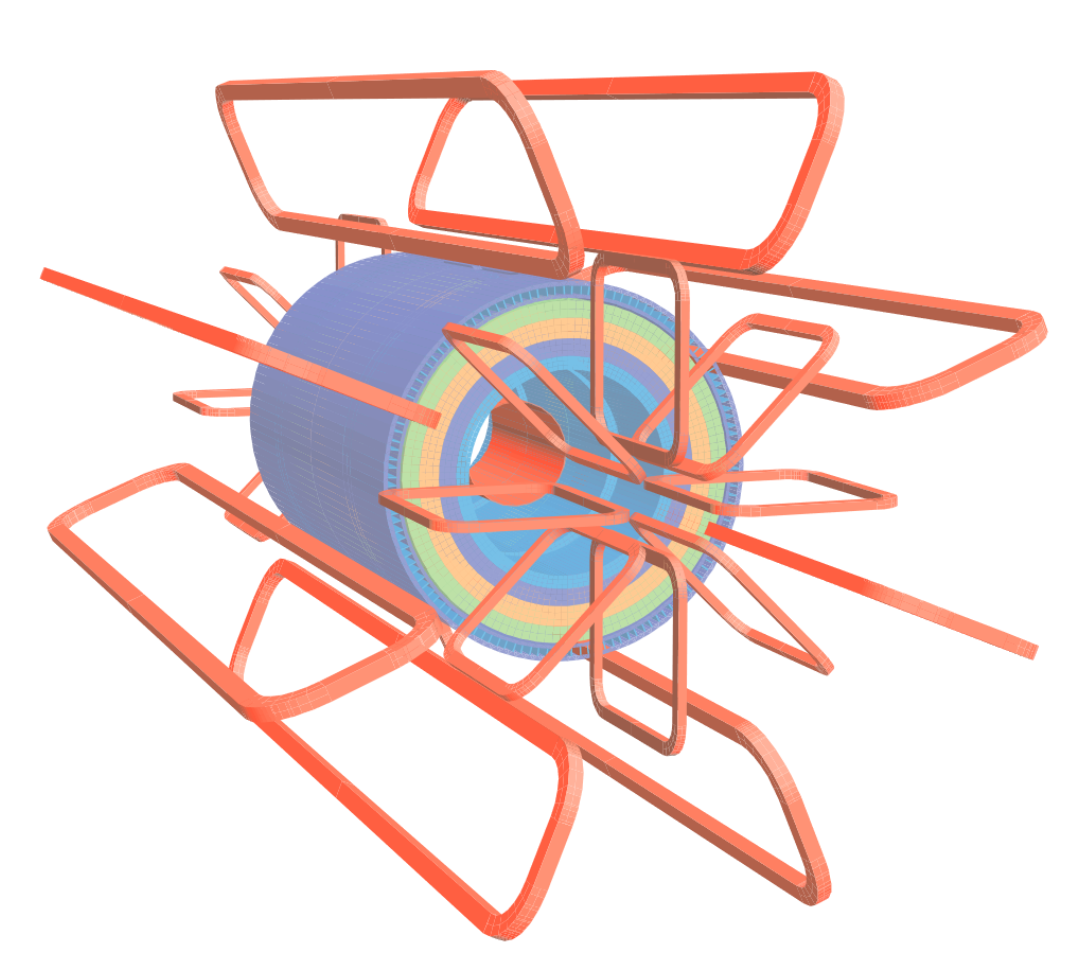
\includegraphics[width=.56\textwidth]{Detector/plots/ATLAS magnets.png}
	\caption{Geometry of magnet windings and
	tile calorimeter steel. Image taken from \cite{PERF-2007-01}.}
	\label{fig:ATLAS_magnets}
	\end{centering}
\end{figure}


\subsection{Inner detector}	
\label{sec:inner detector}
The inner detector (ID) is the closest sub-detector to the
beam line, designed to track the early trajectories of charged particles for
momentum calulations and locat their primary and secondary vertices with
extremely high precision. The ID is required to deal with large numbers of tracks
promptly, where 1000 particle collisions are taking place every 25 ns.  
The ID has full coverage in azimuthal angle $\phi$ and $|\eta|$ < 2.5 acceptance 
in pseudorapidity. As mentioned briefly above, it consists of three parts: 
the pixel detector and the insertable B-Layer (IBL)~\cite{ATLAS-TDR-19} (as one part),
the semiconductor tracker and the transition radiation
tracker. The layout of the ID is shown in figure~\ref{fig:inner_detector},
with a charge track (in red) traversing the sensors and structural elements. 
\begin{figure}[bht]
	\begin{centering}	
	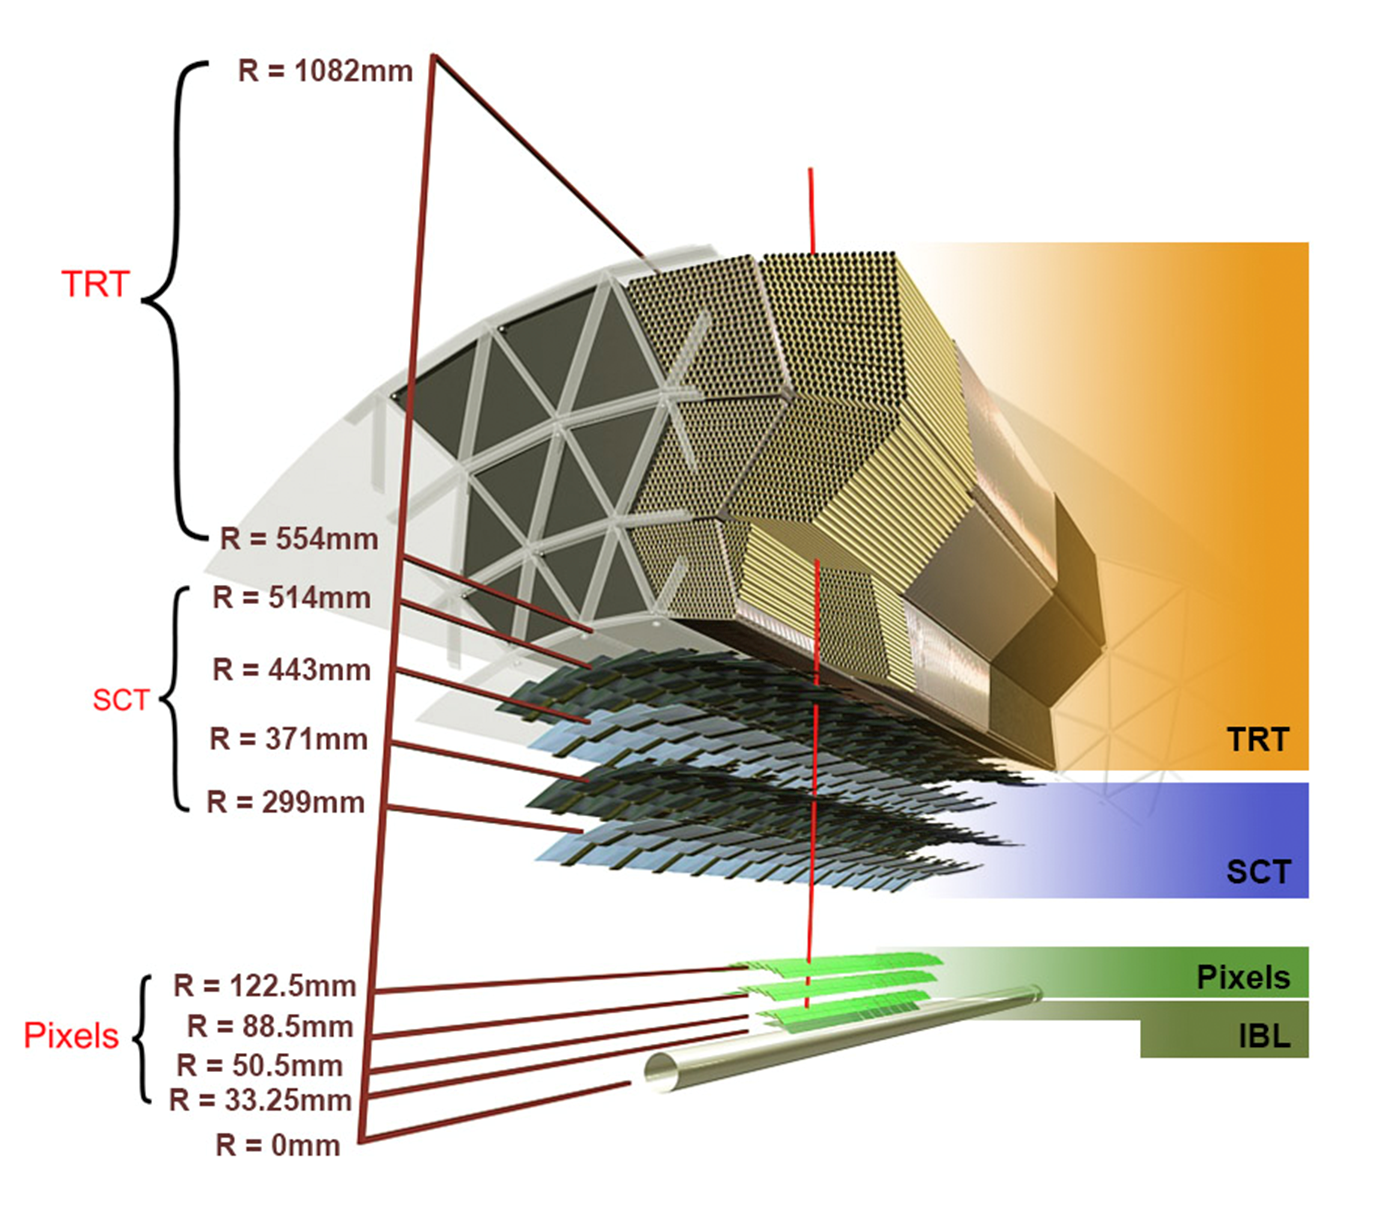
\includegraphics[width=.85\textwidth]{Detector/plots/Inner detector.png}
	\caption{Cut-away view of the inner detector. Image taken from \cite{Pequenao}.}
	\label{fig:inner_detector}
\end{centering}
\end{figure}
% The track traverses successively the beryllium
% beam-pipe, the four cylindrical silicon-pixel layers 
% with individual 
% sensor elements of 50$\times$400 $\mu m^2$, the four cylindrical double 
% layers of barrel SCT of pitch 80 $\mu m$, 
% and approximately 36 axial straws of 4 $mm$ diameter 
% contained in the barrel TRT
% modules within their support structure.
% \begin{itemize}
	\subsubsection{Pixel detector and IBL}
	The silicon pixel detector is the closest ATLAS 
	component to the collision. It is composed of layers of
	silicon pixels and designed to have a very 
	high granularity for reconstructing primary 
	and secondary interaction vertices. 
	The detector layers are formed of silicon sensor modules and 
	in total there are approximately 92~million pixels 
	(consequently, 92~million readout channels) in the system.
	It consists of three cylindrical layers in the 
	barrel region, positioned at the radial distances of 
	50.5, 88.5 and 122.5~mm, 
	and of disks perpendicular to the beams in the end-caps at the
	longitudinal distances of 49.5, 58.0 and 65.0~mm. 
	% The B-layer, placed at a distance of 50.5mm, plays 
	% an important role in detecting secondary vertices 
	% for the identification of jets coming from 
	% b-quark hadronisation (\bjets). 
	In 2014, during the first LHC long shutdown, a fourth pixel 
	layer was installed inside the existing detector, 
	the insertable B-Layer (IBL) at a radius of 33~mm 
	from the beam axis.
	The new pixel layer provides an 
	additional space point very close to the interaction point, 
	which significantly improves the identification of jets coming from 
	$b$-quark hadronisation (\bjets). 
	Particles with $|\eta|$ < 2.5 traverses the four layers usually produce  
	four space-points. The pixel detector provides a resolution of 
	$\sigma_\phi$ = 10 $\mu$m in the bending direction ($R - \phi$), 
	and a resolution of $\sigma$ = 115 $\mu$m in the $z$($R$)
	direction in the barrel (end-cap) region.

	\subsubsection{Semiconductor tracker}
	The next constituent of the inner detector is the SCT. 
	It is a silicon microstrip detector with over six million readout channels, 
	which surrounds the pixel detector and covers the region 
	of radius between 299~mm and 560~mm. 
	It consists of four layers of strips located axially on the 
	beam direction in the barrel region and placed along the 
	$z$-direction in the end-cap region. 
	This configuration allows the particles along the beam pipe
	to be constructed. 
	Each layer of strips is glued back to back with an angle of
	40~mrad to form a two-sided module and make possible the 
	measurement of the second coordinate.
	The sensors are 285 $\mu$m thick and are constructed
	of high-resistivity n-type bulk silicon with p-type implants. 
	Readout strips are positioned every 80 $\mu$m, providing a spatial resolution 
	of $\sigma_\phi = 17\ \mu m$ in the bending direction ($R-\phi$)
	and $\sigma_\phi = 580\ \mu m$ in the z (barrel) and R (end-cap) direction. 

	\subsubsection{Transition radiation tracker}
	The outermost part of the inner detector is the TRT, which covers
	the radial region between 563~mm and 1066~mm. 
	It is a straw drift tube tracker, which consists of
	modules of 4~mm diameter polyimide straws, filled with a mixture of gas of
	70\% Xe, 27\% CO$_2$ and 3\% O$_2$ 
	and a gold-plated tungsten wire in the centre. 
	The straws are interleaved with propylene fibres (foils) in the barrel (end-cap)
	region.
	% All charged tracks with \pt\ $> 0.5$ GeV and $|\eta| < 2.0$ will traverse 
	% at least 36 straws, except in the
	% barrel-end-cap transition region ($0.8 < |\eta|< 1.0$), 
	% where this number decreases to a minimum of 22 crossed straw.
	With a spatial resolution of $\sigma_\phi = 130$ \textrm{$\mu$m}, 
	the TRT measures the track position only in the bending direction
	($R-\phi$). This is because when
	a charged particle passes through a straw tube, electrons from the gas
	are liberated through ionisation; under high voltage, these electrons then drift toward the 
	wire in the certre, where a current flow is created and registered as a hit.
	Since a hit can happen on any location along the wire,
	the information of the $z$ position of the particle is lost. 
	In addition, the TRT provides capability of distinguishing electrons from other
	charged particles. When a highly-relativistic charged particle traverses the
	polymer straws interfacce, the particle emits transition radiation which is then absorbed 
	by the Xeon gas. The intensity of the radiation
	depends on the gamma factor of the particle (strongest for lighter particles), hence this information
	can be exploited for electron identification. 
	% by the particle 
	% The ionisation probability depends on the gamma factor of the charged particle 
	% and hence 
	% The TRT contributes significantly to the pattern recognition and 
	% momentum reconstruction, depsite the low resolution compared to the 
	% silicon tracker and the lack of a measurement along the $z$-axis. 
	% This is the result of the large number of measurements and longer
	% measured track length. In addition, the TRT provides extra ability to 
	% identify elecctrons due to the polypropylene fibres (foils) in the barrel
	% (end-cap) emit photons when a charged particle traverses the boundaries of
	% the material. These photons are then absorbed by the Xenon gas mixture, which
	% the intensity depends on gamma factor of the traversing particle. 
	% This information can then be exploited for electron/pion discrimination.
	% \end{itemize}

\subsection{Calorimeter system}

\label{sec:calorimeter}


Calorimeters are used to measure the energy of both charged and neutral particles. 
The ATLAS calorimeters~\cite{ATLAS-TDR-01}, as shown in Figure~\ref{fig:calo},
are consists of three major components,
the Electromagnetic calorimeter, the Hadronic calorimeter and the Forward calorimeter (FCal).
The fine granularity of the EM calorimeter 
is ideal for precision measurements of electrons and photonsl; the
coarser granularity of hadronic calorimeter is sufficient 
for the hadronic jet reconstruction; the FCal provides coverage of 
large pseudorapidity region: these calorimeters cover the range $|\eta|$< 4.9.
All the three calorimeters are sampling calorimeters. Sampling calorimeters 
use different material the absorber and the active part:
the absorber (or passive material) is reponsible for producing particle showers where 
the active part then measures their energy. Note well the a fraction of
total particles energy deposited in the passive material and it's not
measured; the overall energy must be deduced from the definite
measurements taken in the active detector layers. 

\begin{figure}[bht]
	\begin{centering}	
	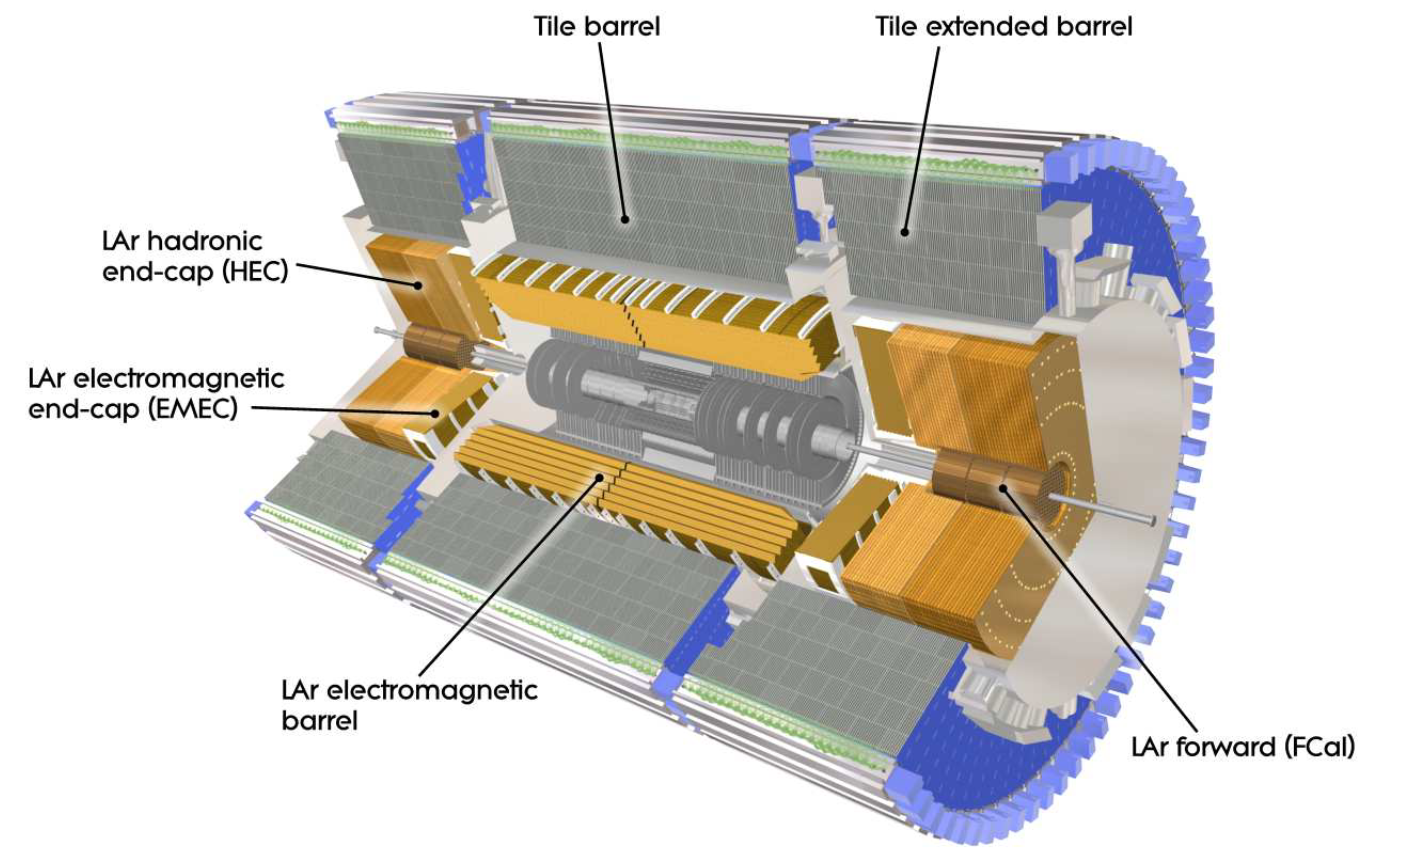
\includegraphics[width=1.0\textwidth]{Detector/plots/calo.png}
	\caption{Cut-away view of the ATLAS calorimeter system. Image taken from~\cite{ATLAS-TDR-01}.}
	\label{fig:calo}
	\end{centering}
\end{figure}
% using different techniques suited to the widely varying requirements 
% of the physics processes of interest and of the radiation environment
% over this large $\eta$-range. 
% over the large $\eta$ region, 
The electromagnetic and hadronic showers must be contained in the 
calorimeter to ensure precise measurement of the total energy of the particle
and to avoid punch-through into the muon system. 
The calorimeter depth is hence an important design consideration. 
The thickness of the calorimeter is measured in radiation length $X_0$,
which is the mean length of a material over which an electron will lose all but $1/e$ 
of its initial energy through radiative processes; and nuclear interaction length $\lambda$,
which is the mean distance travelled by a hadronic particle before undergoing
an inelastic nuclear interaction. 
The total thickness of the EM calorimeter is greater than
22 radiation lengths ($X_0$) in the barrel and greater than 
24 $X_0$ in the end-caps.
% The approximate 9.7 interaction lengths ($\lambda$) of active calorimeter in 
% the barrel ($10\ \lambda$ in the end-caps) are adequate to 
% provide good resolution for high-energy jets.
The total thickness of the calorimeters, 
including $1.3\ \lambda$ from the outer support, is $11\ \lambda$
at $\eta$ = 0 and has been shown both by measurements and simulations 
to be sufficient to reduce punch-through well below the irreducible 
level of prompt or decay muons. 
% Together with the large
% \mbox{$\eta$-coverage}, this thickness will also ensure a good $E_{miss}^T$ 
% measurement.


	\subsubsection{Electromagnetic calorimeter} 
	The EM calorimeter is a lead-Liquid argon (lead-LAr) detector~\cite{ATLAS-TDR-02} 
	with accordion-shaped (as shown in Figure~\ref{fig:accordion}) kapton electrodes and lead 
	absorber plates over its full coverage, while using liquid argon (LAr) as the active 
	material. 
	% The accordion geometry provides complete $\phi$ symmetry without azimuthal cracks. 
	The lead thickness in the absorber plates has been optimised as a function of $\eta$ 
	in terms of EM calorimeter performance in energy resolution. 
	The EM calorimeter is divided into a barrel part ($|\eta| < 1.475$) 
	and two end-cap components ($1.375 < |\eta|< 3.2$), each housed 
	in their own cryostat. Additional material needed to instrument
	and cool the detector creates a ``crack'' region at $1.375 < |\eta|< 1.52$, where the 
	energy resolution is significantly degraded.
	
	\begin{figure}[bht]
		\begin{centering}	
		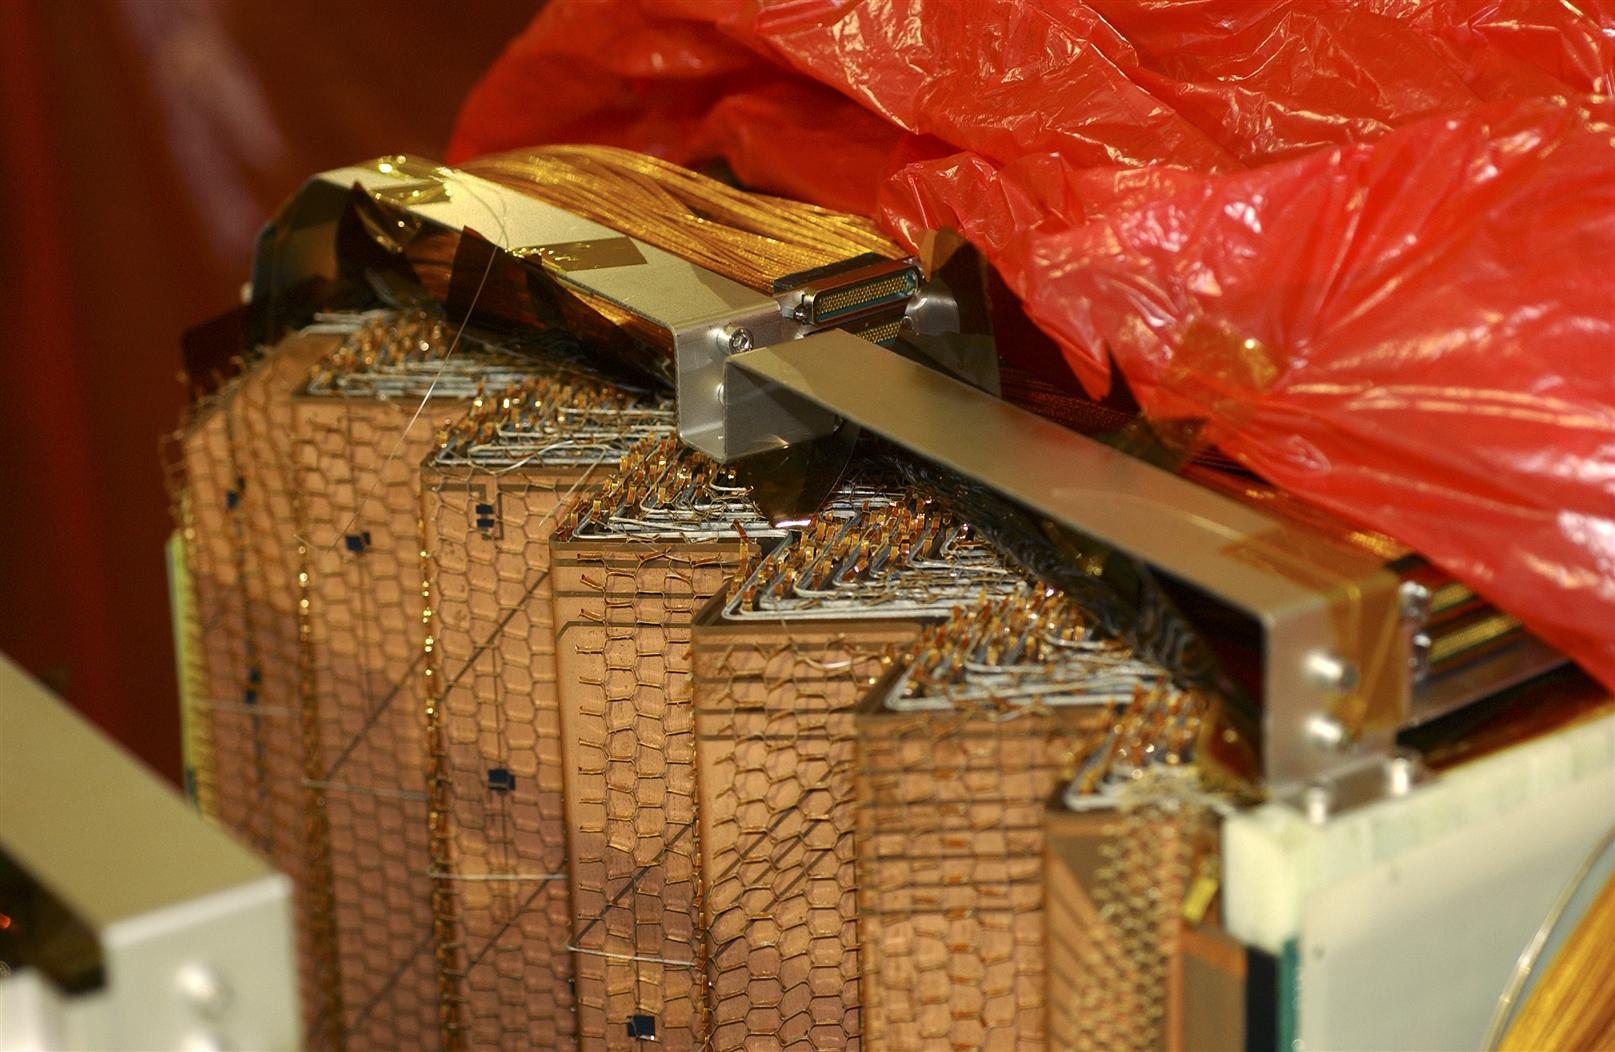
\includegraphics[width=.6\textwidth]{Detector/plots/accordion.jpg}
		\caption{A figure of the accordion-shaped electrodes.}
		\label{fig:accordion}
		\end{centering}
	\end{figure}
	%  The position of the central solenoid in
	% front of the EM calorimeter demands optimisation of the material 
	% in order to achieve the desired calorimeter performance. As a consequence, 
	% the central solenoid and the LAr calorimeter share a common vacuum vessel, 
	% thereby eliminating two vacuum walls. 
	The barrel calorimeter 	consists of two identical half-barrels, 
	separated by a small gap (4~mm) at $z$ = 0. 
	Each end-cap calorimeter is mechanically divided into two coaxial wheels: 
	an outer wheel covering the region $1.375 < |\eta|< 2.5$, and an inner wheel 
	covering the region $2.5 < |\eta|< 3.2$.
	
	The calorimeter has three layers along the transverse direction:
	a pre-sampler with very high granularity in $\eta$, in order to 
	reconstruct the neutral pions decaying to two photons and particles 
	which already starts showering in the inner detector. 
	The pre-sampler is followed by longer towers of relatively 
	high granularity, which is the major part of detecting EM showers, 
	and reponsible for measuring the $\eta$ and $\phi$ coordinates of 
	the particles. The last layer detects showers generated from 
	particles other than electrons or photons that start showering 
	inside the EM calorimeter before leaving it.

	\subsubsection{Hadronic calorimeter}
	The Hadronic calorimeter is comprised of the Tile Hadronic calorimeter (HCAL) 
	and the LAr hadronic end-cap calorimeter (HEC). 
	The HCAL is placed directly outside the EM calorimeter envelope. 
	Its	barrel covers the region $|\eta|< 1.0$, and its two extended barrels 
	the range $0.8 < |\eta|< 1.7$. It is using steel as the absorber and scintillating tiles
	as the active material. 
	% The	barrel and extended barrels are divided azimuthally into 64~modules. 
	% Radially, the tile calorimeter
	% extends from an inner radius of 2.28~m to an outer radius of 4.25~m. 
	It is segmented in depth in three layers, approximately 1.5, 4.1 and 1.8 $\lambda$ 
	thick for the barrel and 1.5, 2.6, and 3.3 $\lambda$ for the extended barrel. 
	The total detector thickness at the outer edge of the tile-instrumented
	region is 9.7 $\lambda$ at $\eta$ = 0. 
	% Two sides of the scintillating tiles are read out by wavelength shifting
	% fibres into two separate photomultiplier tubes. 
	% In $\eta$, the readout cells built by grouping fibres into
	% the photomultipliers are pseudo-projective towards the interaction region.
	
	The HEC is similar to the construction to the ECAL, using LAr as the 
	active material, but instead of using lead it uses copper as the absorber.
	It consists of two independent wheels per end-cap, located directly 
	behind the end-cap electromagnetic calorimeter and sharing the same LAr cryostats. 
	The HEC covers the range of $1.5< |\eta|< 3.2$, 
	slightly overlapping with the forward calorimeter which 
	will be described in the following paragraph 
	(around $|\eta|$= 3.1) and the tile calorimeter ($|\eta|< 1.7$).
	This overlap is to reduce the drop in material density at the transition between
	the different calorimeters.
	% Each wheel is built from 32
	% identical wedge-shaped modules, assembled with fixtures at the periphery 
	% and at the central bore.
	% Each wheel is divided into two segments in depth, for a total of four 
	% layers per end-cap. The wheels
	% closest to the interaction point are built from 25~mm parallel copper plates, 
	% while those further away
	% use 50~mm copper plates (for all wheels the first plate is half-thickness). 
	% The outer radius of the
	% copper plates is 2.03~m, while the inner radius is 0.475~m 
	% (except in the overlap region with the
	% forward calorimeter where this radius becomes 0.372~m). 
	% The copper plates are interleaved with
	% 8.5~mm LAr gaps, providing the active medium for this sampling calorimeter.
	\subsubsection{Forward calorimeter}
	The Forward Calorimeter (FCal) covers $3.1 < |\eta| < 4.9 $ and
	%  is integrated into the end-cap cryostats, 
	% as this provides clear benefits in terms of uniformity of the calorimetric 
	% coverage as well as reduced radiation background levels in the muon spectrometer. 
	% In order to reduce the amount of neutron albedo in the inner detector cavity, 
	% the front face of the FCal is recessed by about 1.2~m with respect to the EM calorimeter 
	% front face. This severely limits the depth of the calorimeter
	% and therefore calls for a high-density design. The FCal 
	is approximately 10 interaction lengths deep. 
	It consists of three modules in each end-cap: 
	the first, made of copper, is optimised for	electromagnetic measurements, 
	while the other two, made of tungsten, measure predominantly the
	energy of hadronic interactions. All three modules use LAr as active material.
	Due to high particle fluxes andenergies in the forward region, 
	the calorimeter must contain relatively long showers 
	in the small volume allowed by design constraints, 
	and thus must be very dense.
	% Each module consists of a metal matrix, 
	% with regularly spaced longitudinal channels filled with the electrode structure 
	% consisting of concentric rods and tubes	parallel to the beam axis. 
	% The LAr in the gap between the rod and the tube is the sensitive medium.
	% This geometry allows for excellent control of the gaps, which are as small 
	% as 0.25~mm in the first
	% section, in order to avoid problems due to ion buildup. 



\subsection{Muon Spectrometer}
\label{sec:MS}
The muon spectrometer is the outermost and largest sub-detector of ATLAS. 
A cut-away view of the MS is illustrated in Figure~\ref{fig:MS}.
It fully covers the	calorimeter system and occupies a large part of the ATLAS cavern. 
It is based on the magnetic deflection of muon tracks in the 
large superconducting air-core toroid magnets, instrumented with
separate trigger and high-precision tracking chambers. 
Over the range $|\eta|< 1.4$, magnetic bending is provided by the large 
barrel toroid. For $1.6 < |\eta|< 2.7$, muon tracks are bent by two smaller
end-cap magnets inserted into both ends of the barrel toroid. 
Over $1.4 < |\eta|< 1.6$, usually referred to as the transition region, 
magnetic deflection is provided by a combination of barrel and end-cap
fields. The configuration of magnets provides a field mostly orthogonal 
to the muon trajectories, hence minimising the degradation of 
resolution due to multiple scattering. 
% The anticipated high level of 
% particle flux has had a major impact on the choice and design of the spectrometer 
% instrumentation, affecting performance parameters such as rate capability, granularity, ageing
% properties, and radiation hardness.
% In the barrel region, tracks are measured in chambers arranged in three cylindrical layers
% around the beam axis; in the transition and end-cap regions, the chambers are installed in planes
% perpendicular to the beam, also in three layers.
\begin{figure}[bht]
	\begin{centering}	
	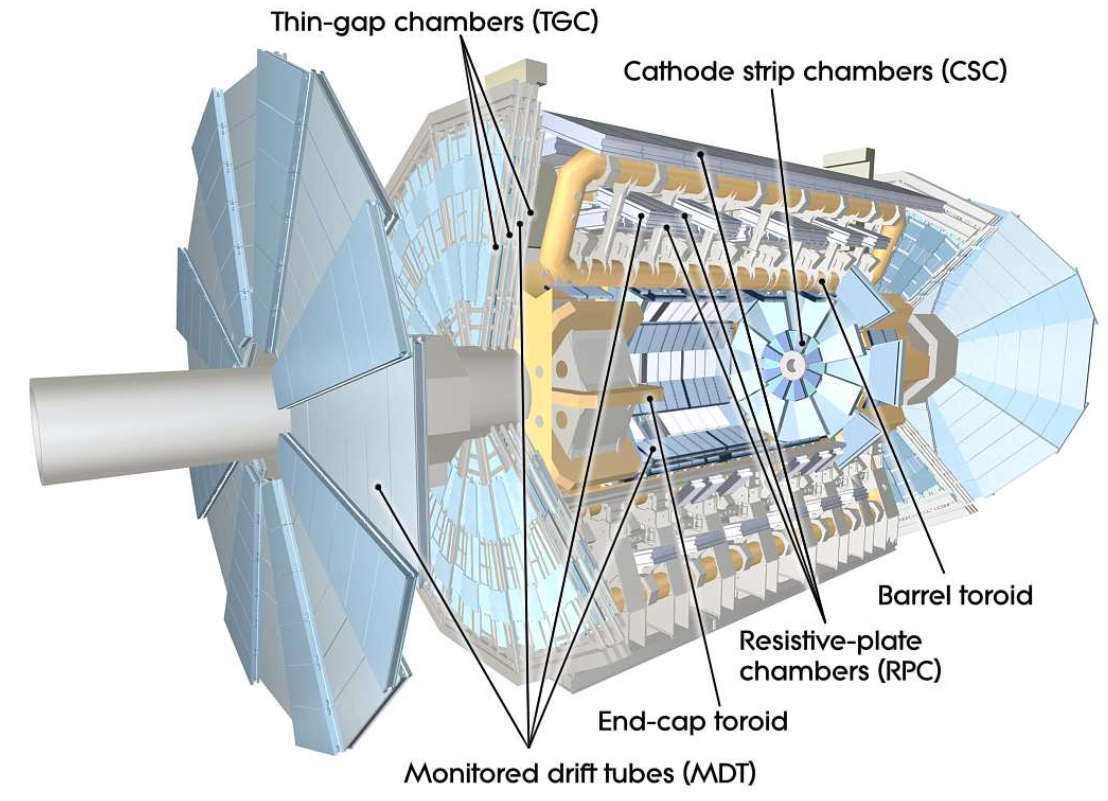
\includegraphics[width=.9\textwidth]{Detector/plots/Muon.png}
	\caption{Cut-away view of the ATLAS muon spectrometer system. Image taken from \cite{PERF-2007-01}.}
	\label{fig:MS}
	\end{centering}
\end{figure}

The MS consists of four subsystems which rely on four different gas detector
technologies. Two of them, the resistive plate chambers (RPC) in the barrel region 
and the thin gap chambers (TGC) in the end-cap region, provide trigger signals, 
while the other two, the monitored drift tubes (MDT) in the barrel and the cathode strip 
chambers (CSC) in the end-cap region provide the momentum measurement. 
The MDT chambers provide high precision measurements in the bending direction over most of the detector
acceptance while the CSC are used in the forward region where the particle flux 
is too high for the MDT	chambers. The muon chambers are arranged in the barrel 
($|\eta| < 1.05$) in three cylindrical layers around the beam axis, 
while in the end-cap regions ($1.05 < |\eta| < 2.7$) they are placed in three wheels.
The resolution of muons tracks momentum measurement varies from typically 2–3\% over
most of the kinematic range, to about 10\% at \pt\ = 1 TeV.  

\subsection{Trigger system}
\label{sec:ATLAS:trigger}
% \begin{figure}[bht]
% 	\begin{centering}	
% 	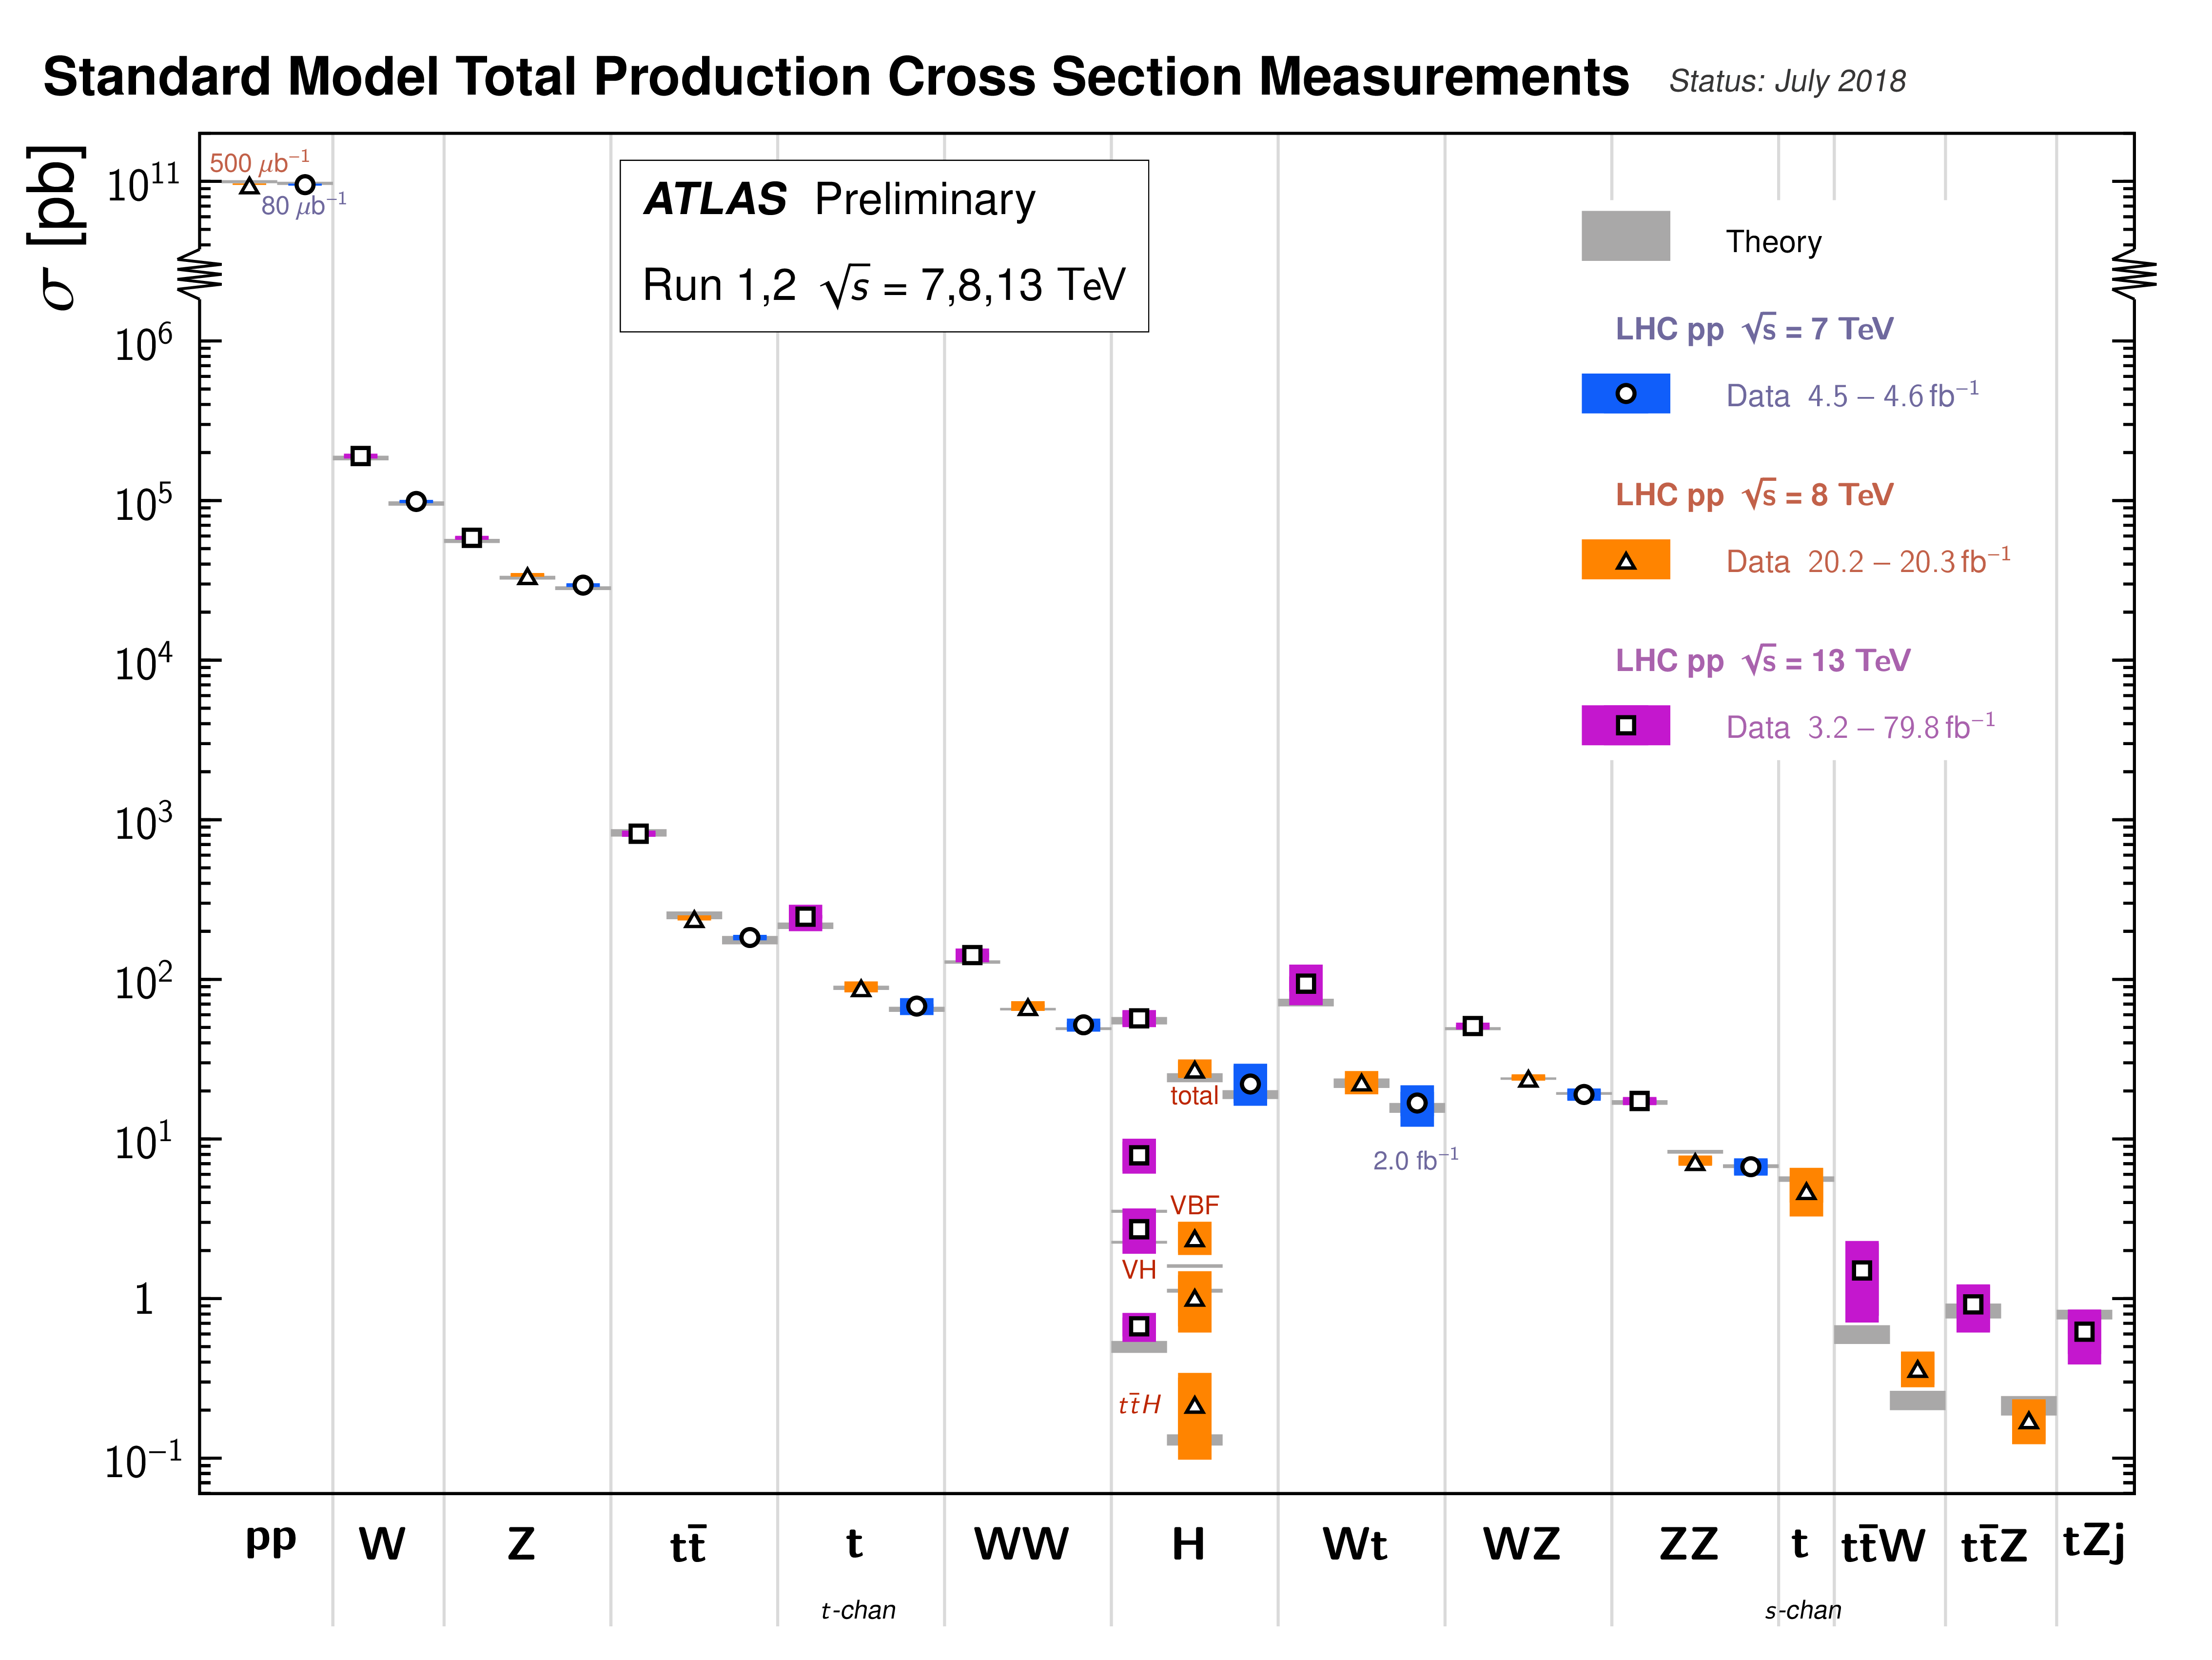
\includegraphics[width=.97\textwidth]{Detector/plots/summary xs.png}
% 	\caption{Plot showing the production cross-sections of the most dominant
% 	background processes at the LHC.}
% 	\label{fig:summary production Xs}
% 	\end{centering}
% \end{figure}
As mentioned in section \ref{sec:Operation schedule}, the spacing of each bunch
is 25 ns, which translates to a 40~MHz of bunch-crossing frequency, with up to 80
collisions per bunch crossing. This is far beyond the data collection bandwidth and 
storage capacity of ATLAS. 
% will be difficult and not meaningful to keep all these events, which includes
% a lot of ``uninteresting'' physics events. Figure~\ref{fig:summary production Xs} 
% shows a summary of the most dominant background processes production cross-sections.
% Many of these processes produce high multiplicity of jets and are not of experimental
% interest. 
Therefore, it's necessary to adopts a trigger system that make fast decisions
whether an event is high quality, rare or ``interesting'' and to save the event or not.
The ATLAS trigger system consists of two consecutive parts: the Level 1 trigger~\cite{ATLAS-TDR-12}
which is hardware-based, 
followed by the the software-based High Level Trigger (HLT)~\cite{ATLAS-TDR-16}.

The L1 trigger searches for signatures from high-\pt\ muons, electrons/photons, jets, and 
\mbox{$\tau$-leptons} decaying into hadrons. It also selects events with large MET
and large total transverse energy. The L1 trigger uses reduced-granularity information from a
subset of detectors: the RPC and TGC for high-\pt\ muons, and all the calorimeter 
sub-systems for electromagnetic clusters, jets, $\tau$-leptons, $E_{miss}^T$ ,
and large total transverse energy.
As a result, the L1 trigger reduces the event rate from 40~MHz to a maximum of 100 kHz.
The decision is made by Central Trigger	Processor (CTP), 
which operates on signals from dedicated hardware in the calorimeter
and muon detector systems. The decision time, at under 2.5 $\mu s$, is faster than the ID
can process events so ID information is omitted.
For each data-taking period, the L1	trigger is loaded with a trigger menu, 
a list of up to 256 criteria used to determine
whether an event is accepted. The trigger menus are designed to accomodate a broad
physics programme, with high acceptance for both BSM searches and SM precision
measurements.
The L1 trigger also uses detector information with reduced granularity to identify Regions
of Interest (RoI)~\cite{Blair:2007qn} in $\phi$ and $\eta$.
The ROI information with full granularity and precision and all the available detector 
data (including the ID information) within the RoI's are provided to the HLT. 
% The HLT menus are designed to reduce the
% trigger rate to approximately 3.5 kHz, with an event processing time of about 40~ms,
% averaged over all events. 
% The final stage of the event selection is carried out by 
% the event filter, which reduces the event rate to roughly 200 Hz. 
% The selections are implemented using offline analysis procedures
% within an average event processing time of the order of four seconds.
% These events are stored and processed for later analysis. 
This trigger level reduces the rate of events by two orders of magnitude,
reaching an average of 1 kHz with a latency of 0.2 $\mu$s.
These events are passed on to a data storage system for offline analysis.

